\documentclass[12pt,a4paper]{article}
\usepackage[utf8]{inputenc}
\usepackage{graphicx}
\usepackage{geometry}
\usepackage{hyperref}
\usepackage{booktabs}
\usepackage{float}
\geometry{a4paper, margin=1in}

\title{Unsupervised Learning Project: Autoencoders on MNIST \texorpdfstring{\\[0.5em]}{ - }
\texorpdfstring{\large }{ }Project Report}
\author{Ahmet Enes Çiğdem (150220079) - Team Leader \and Mehmet Akif Dündar (150220015)}
\date{\today}

\begin{document}

\maketitle

\section{Introduction}
This report details the implementation, training, and evaluation of an autoencoder neural network for unsupervised representation learning on the MNIST dataset. In this updated study, we extend our analysis to compare different sizes of the latent space bottleneck ($16$, $32$, and $64$ dimensions), incorporating modern regularization techniques such as Batch Normalization, and observing the subsequent effects on reconstruction loss and clustering performance (K-Means).

\section{Architecture of the Autoencoder}
The autoencoder is constructed using fully connected (linear) layers, partitioned into an encoder and a symmetric decoder. To stabilize training over 50 epochs and accelerate convergence, Batch Normalization layers were integrated before activation functions.
\begin{itemize}
    \item \textbf{Latent Space Size:} Evaluated across 3 configurations: $16$, $32$, and $64$.
    \item \textbf{Encoder Structure:}
    \begin{enumerate}
        \item Linear Layer (784 $\rightarrow$ 256) $\rightarrow$ \texttt{BatchNorm1d(256)} $\rightarrow$ \texttt{ReLU}
        \item Linear Layer (256 $\rightarrow$ 64) $\rightarrow$ \texttt{BatchNorm1d(64)} $\rightarrow$ \texttt{ReLU}
        \item Linear Layer (64 $\rightarrow$ \texttt{latent\_dim}) without an activation function to allow unrestricted, continuous representations.
    \end{enumerate}
    \item \textbf{Decoder Structure:}
    \begin{enumerate}
        \item Linear Layer (\texttt{latent\_dim} $\rightarrow$ 64) $\rightarrow$ \texttt{BatchNorm1d(64)} $\rightarrow$ \texttt{ReLU}
        \item Linear Layer (64 $\rightarrow$ 256) $\rightarrow$ \texttt{BatchNorm1d(256)} $\rightarrow$ \texttt{ReLU}
        \item Linear Layer (256 $\rightarrow$ 784) $\rightarrow$ \texttt{Sigmoid} to ensure output pixel intensities scale correctly within a [0, 1] range.
    \end{enumerate}
\end{itemize}

\section{Training Process}
The models were trained over 50 epochs utilizing the Adam Optimizer with a learning rate of $1 \times 10^{-3}$, a batch size of 256, and Mean Squared Error (MSE) as the loss criterion.

\textbf{Challenge Analysis:} 
The fundamental challenge consisted of finding the optimal dimensional bottleneck. A strict bottleneck (16) forces the model to heavily compress semantic features, hurting pixel-perfect reconstruction but theoretically preserving clustered density. A loose bottleneck (64) vastly improves perfect visual reconstruction (lowest loss) but suffers from the "curse of dimensionality" when running traditional K-Means clustering, preventing it from isolating generalized digit patterns.

\begin{figure}[H]
    \centering
    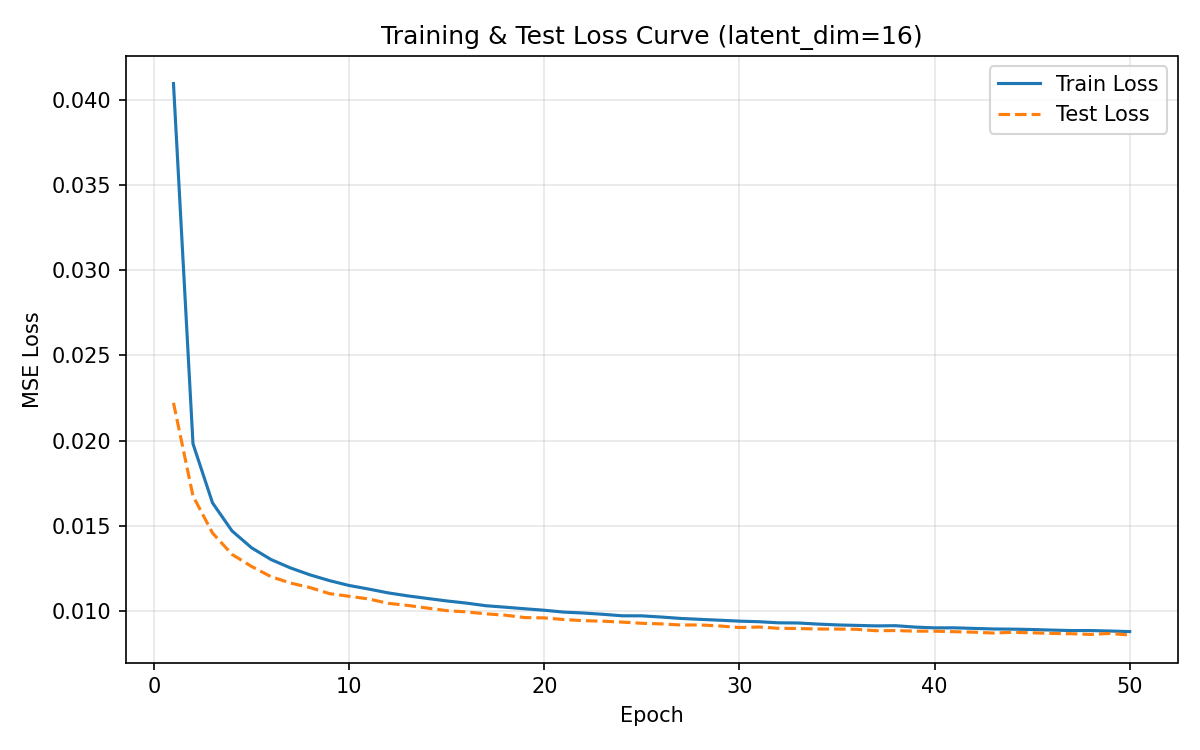
\includegraphics[width=0.7\textwidth]{../results/latent_16/loss_curve.png}
    \caption{Training and Test Loss Curves for the baseline $latent\_dim = 16$ over 50 epochs.}
    \label{fig:loss_16}
\end{figure}

\section{Clustering Performance and Comparison}
To objectively evaluate the representations, K-Means clustering ($k=10$) was applied directly to the extracted high-dimensional latent space. Due to K-Means operating independently from real classes, a Hungarian matching algorithm was used to associate the unsupervised clusters to their most likely true digit labels.

The performance scaling across latent dimensions reveals a classic trade-off:

\begin{table}[H]
    \centering
    \begin{tabular}{lrrr}
        \toprule
        \textbf{Metric} & \textbf{Latent 16} & \textbf{Latent 32} & \textbf{Latent 64} \\
        \midrule
        Final Train Loss (MSE)      & 0.0088      & 0.0051      & \textbf{0.0036} \\
        Final Test Loss  (MSE)      & 0.0086      & 0.0050      & \textbf{0.0035} \\
        % PMS is Percentage of Mislabeled Samples
        PMS (\%)                    & \textbf{36.48}       & 41.93       & 45.44 \\
        Average Distance (AD)       & \textbf{9.7564}      & 11.4930     & 13.8231 \\
        Average Variance (AVC)      & \textbf{9.5422}      & 11.2179     & 13.5350 \\
        Total Distance (TD)         & \textbf{764.8365}    & 514.6528    & 405.9555 \\
        \bottomrule
    \end{tabular}
    \caption{Experimental Results across Latent Dimensions. Bold highlights maximum performance.}
    \label{tab:comparison}
\end{table}

\textbf{Analysis:} While increasing the latent dimensionality to 64 allows the decoder to produce near-perfect visual reconstructions (lowest MSE), it severely degrades K-Means clustering (45.44\% mislabeling rate vs 36.48\% at dim=16). In 64-dimensional space, data becomes sparse, average variance (AVC) expands, and global separation between cluster centers (TD) shrinks, making unsupervised grouping significantly harder. Therefore, $latent\_dim = 16$ presents the best structural embedding for unsupervised clustering. 

\section{Visualizations (Latent Dim = 16)}

\subsection{Reconstruction Quality}
\begin{figure}[H]
    \centering
    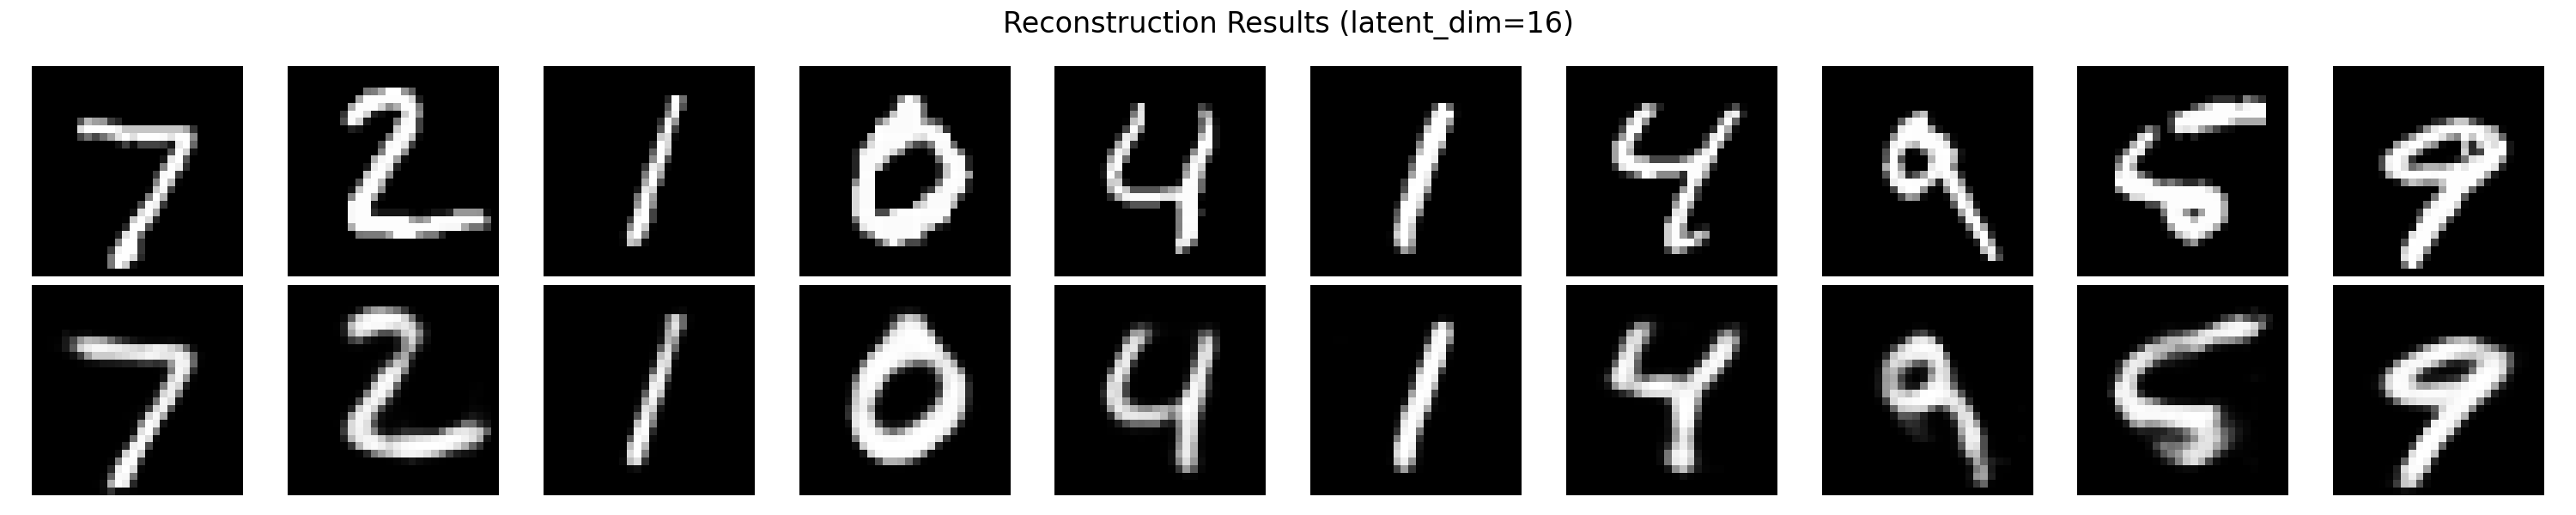
\includegraphics[width=1\textwidth]{../results/latent_16/reconstructions.png}
    \caption{Original Images (Top) vs. Reconstructed Images (Bottom) at 16 dimensions.}
    \label{fig:reconstruction}
\end{figure}

\subsection{Latent Space Projections}
Dimensionality reduction models (PCA and t-SNE) extracted and projected the 16-dimensional coordinates onto an interpretable 2D grid. The plots represent points colored by their True Labels.

\begin{figure}[H]
    \centering
    \begin{minipage}{0.48\textwidth}
        \centering
        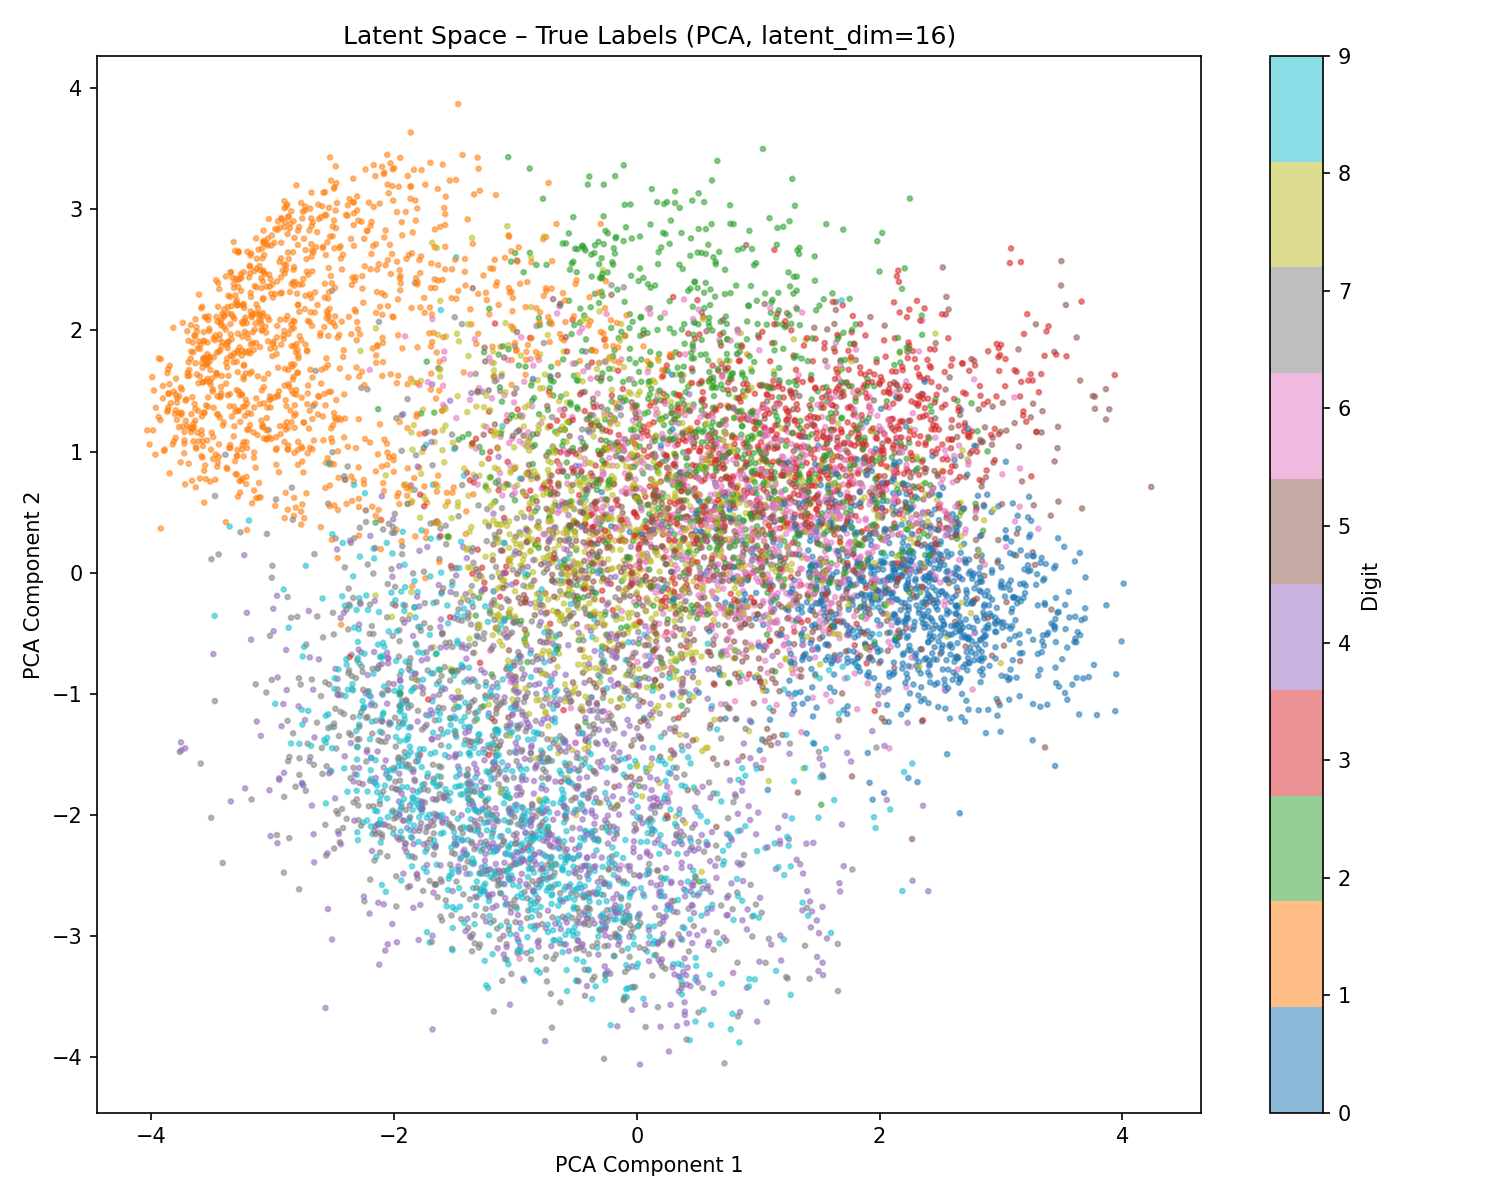
\includegraphics[width=\textwidth]{../results/latent_16/latent_space_pca_true.png}
        \caption{PCA Projection}
    \end{minipage}\hfill
    \begin{minipage}{0.48\textwidth}
        \centering
        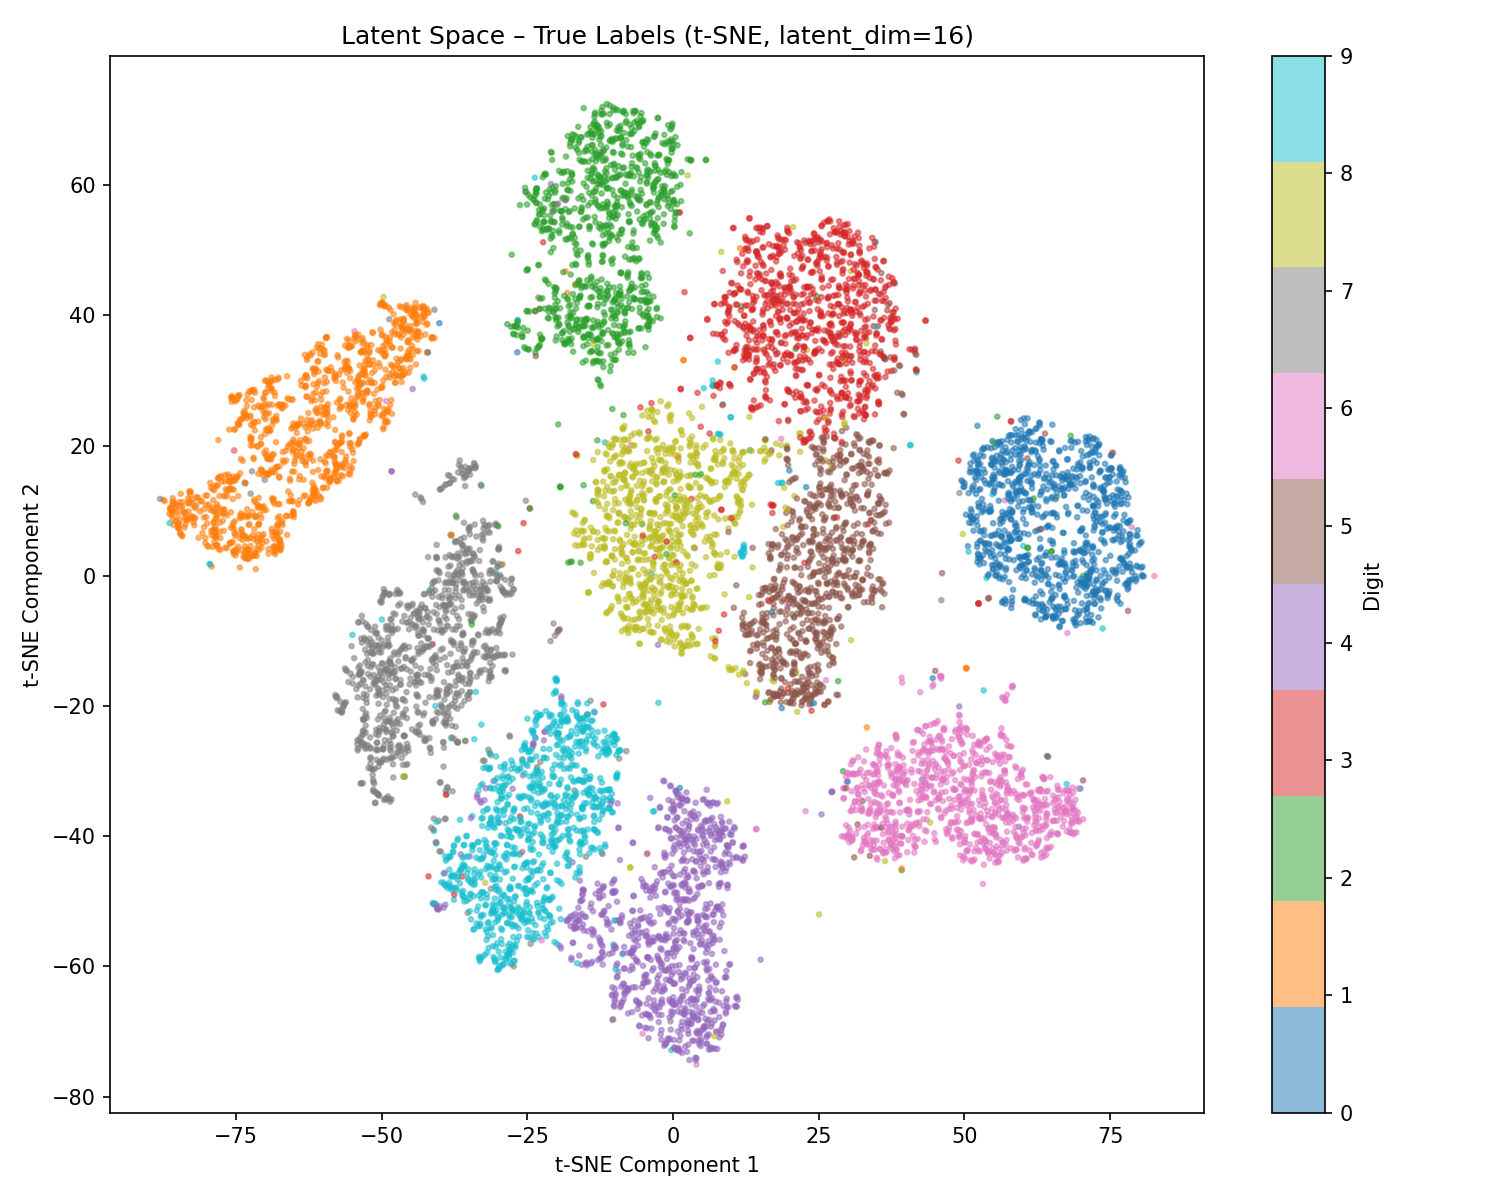
\includegraphics[width=\textwidth]{../results/latent_16/latent_space_t-sne_true.png}
        \caption{t-SNE Projection}
    \end{minipage}
\end{figure}

Due to the non-linear relationship optimized by t-SNE, it successfully maps functionally similar semantic numbers far closer than linear PCA.

\subsection{Confusion Matrix}
\begin{figure}[H]
    \centering
    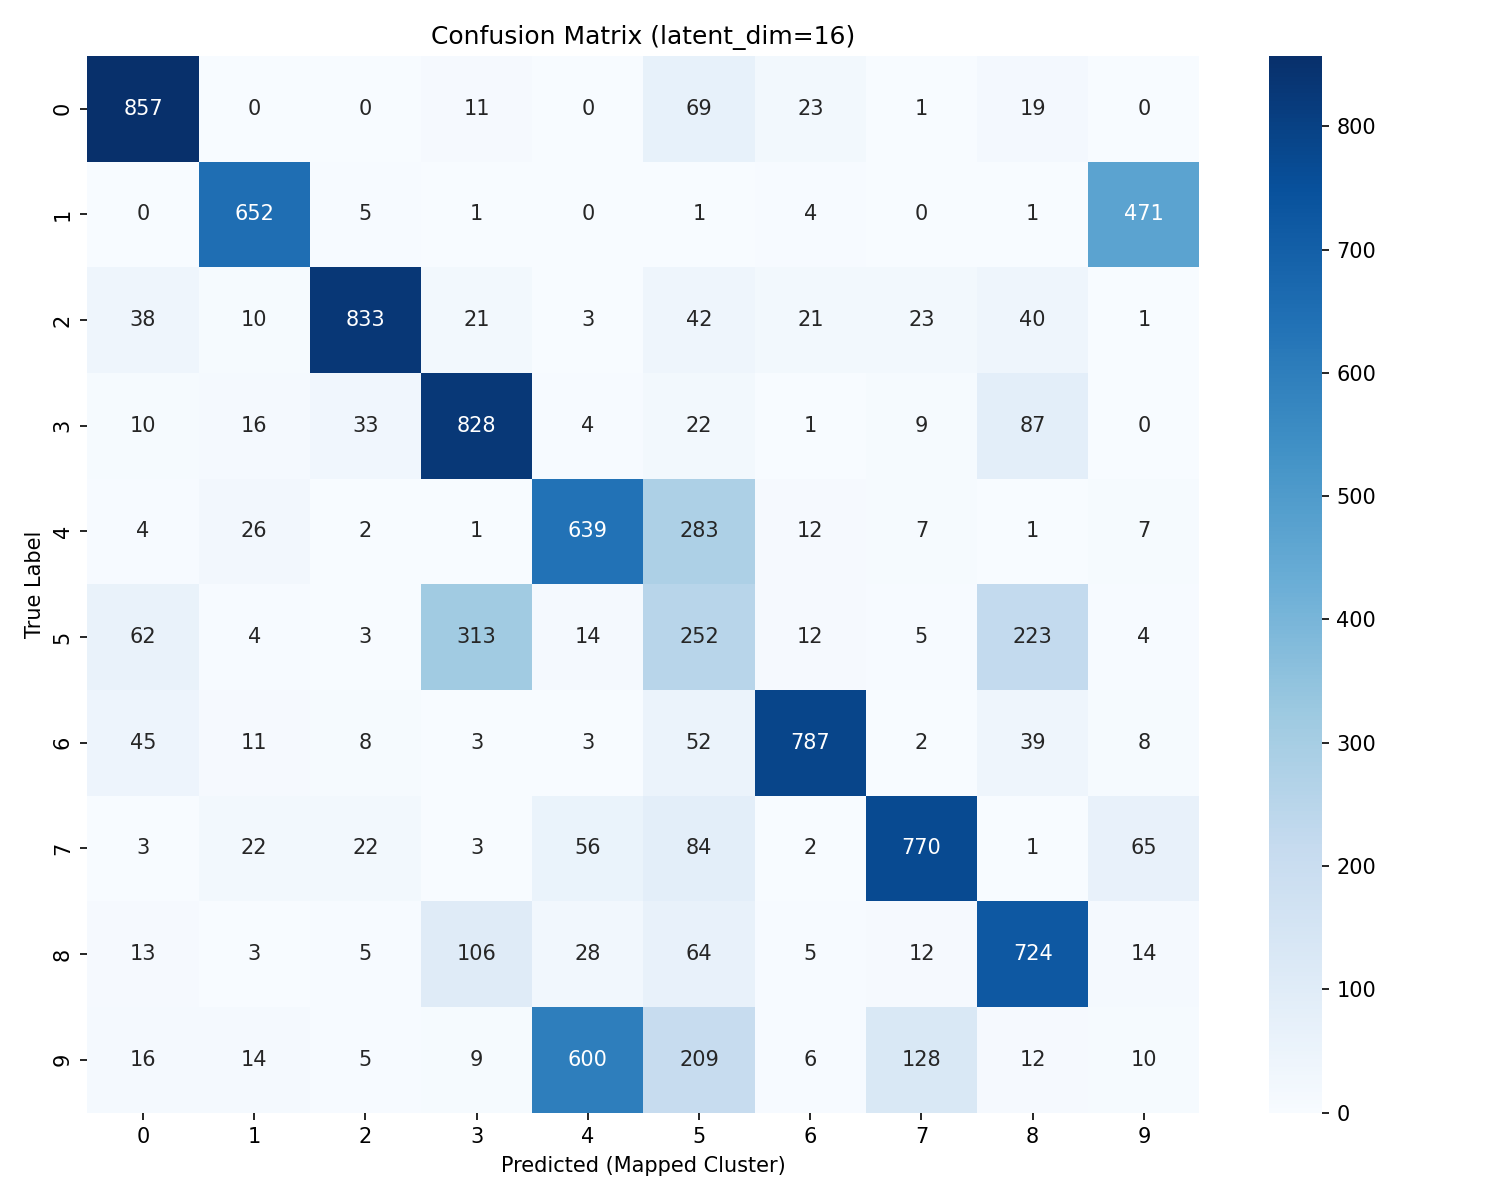
\includegraphics[width=0.6\textwidth]{../results/latent_16/confusion_matrix.png}
    \caption{Confusion Matrix mapping K-Means unsupervised clusters to True Labels.}
    \label{fig:cm}
\end{figure}
A densely populated diagonal demonstrates that the autoencoder grouped unique digit stroke shapes into confined sectors inside the 16-dimensional manifold before the label assignment was enforced.

\end{document}
